\section{自热式固定床反应器}


\begin{frame}
    \frametitle{自热式固定床反应器}

    自热式固定床反应器是换热式固定床反应器的一种特例
    \begin{itemize}
        \item 以原料气作为冷却剂来冷却床层
        \item 将原料气预热至反应所要求的温度，然后进入床层反应。
        \item 只适用于放热反应且原料气必须预热的系统
        \item 反应物料和换热介质的流向对过程的换热起重要的作用
    \end{itemize}

\end{frame}


\begin{frame}
    \frametitle{逆流情况}

        \begin{minipage}{0.4\linewidth}
            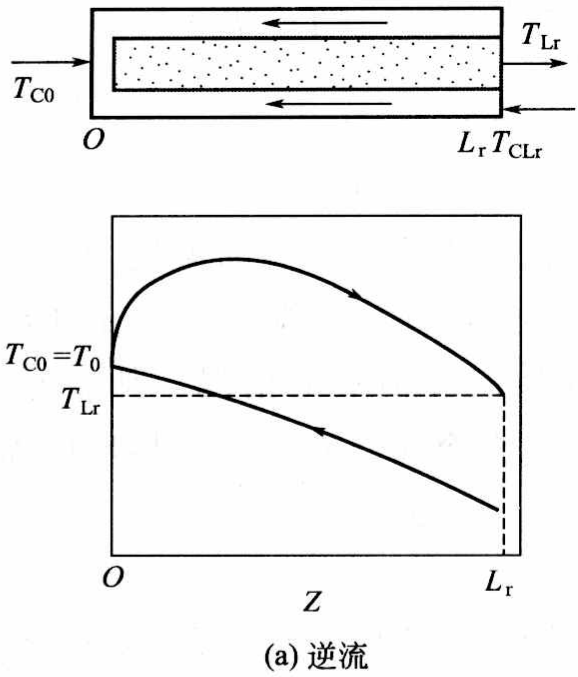
\includegraphics[width=\linewidth]{figures/fig7.9a.png}
        \end{minipage}\hfill
        \begin{minipage}{0.58\linewidth}
            \begin{itemize}
                \item 床层入口处附近的区域，反应物浓度高，放热速率最大
                \item 床层入口处管外气体温度较高
                \item 传热温度差小，管内气体温度上升快
                \item 管内气体温度很快就升高至热点温度
                \item 反应后期传热温度差太大，以致容易出现过冷现象。
            \end{itemize}
        \end{minipage}

\end{frame}


\begin{frame}
    \frametitle{并流情况}

        \begin{minipage}{0.4\linewidth}
            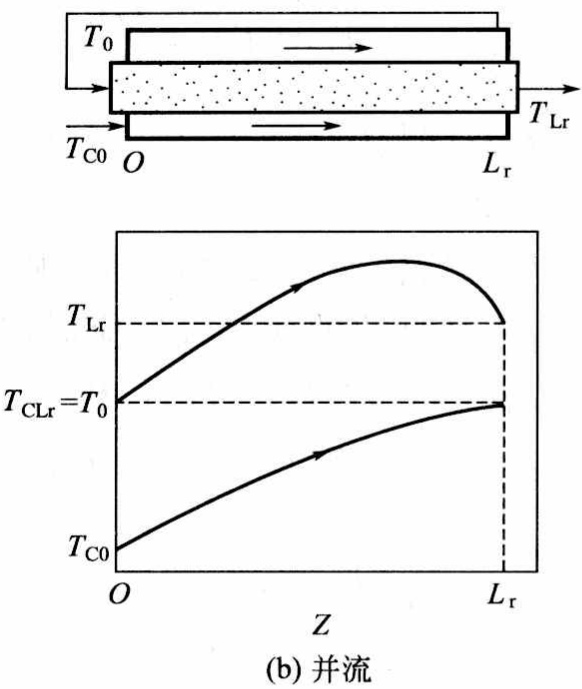
\includegraphics[width=\linewidth]{figures/fig7.9b.png}
        \end{minipage}\hfill
        \begin{minipage}{0.58\linewidth}
            \begin{itemize}
                \item 反应前期，床层内气体升温速度慢。
                \item 反应后期，降温较慢，使床层温度不致太低。
            \end{itemize}
            如何优化？
            \begin{itemize}
              \item 有些并流式催化反应器中设置一绝热床 ， 经预热后的原料气先进入绝热床中反应 ， 使反应气体迅速升温 ， 然后再进入与原料气进行换热的催化剂管中反应 。
            \end{itemize}
        \end{minipage}

\end{frame}


\begin{frame}
    \frametitle{数学模拟}

    由于以原料气作为冷却介质，具体应用固定床反应器数学模型时需对热量衡算式作些改写。

    热量衡算：
    \[
        \frac{G w_{\mathrm{A} 0}}{M_{\mathrm{A}}}(-\Delta H_{\mathrm{r}}) X_{\mathrm{A}}=G \bar{C}_{p \mathrm{t}}(T-T_{0})+G_{\mathrm{C}} \bar{C}_{p \mathrm{c}}(T_{\mathrm{C}}-T_{\mathrm{C} 0})
    \]
    令$G \bar{C}_{p\mathrm{t}} / G_{\mathrm{C}} \bar{C}_{p \mathrm{c}}=\beta$，化简后得
    \[
        T_{\mathrm{C}}=T_{\mathrm{C} 0}+\beta(\lambda X_{\mathrm{A}}-T+T_{0})
    \]
    \vspace{-16pt}
    \begin{itemize}
        \item $\beta = 1$，$G \bar{C}_{p\mathrm{t}} = G_{\mathrm{C}} \bar{C}_{p \mathrm{c}}$，即原料气为冷却介质，为自热反应器。
        \item $\beta = 0$，$T_{\mathrm{C}}=T_{\mathrm{C} 0}$，相当于冷却介质温度恒定的情况。
        \item $\beta \to \infty$，$G_{\mathrm{C}}=0$，属于绝热反应
    \end{itemize}

\end{frame}


\begin{frame}
    \frametitle{数学模拟}

    自热反应器：
    \[
        T_{\mathrm{C}}=T_{\mathrm{C} 0} \pm (\lambda X_{\mathrm{A}}-T+T_{0})
    \]
    并流时取正号，并流式自热反应器床层轴向温度分布微分方程为
    \[
        G C_{p \mathrm{t} } \frac{\mathrm{d} T}{\mathrm{d} Z}=(-\Delta H_{\mathrm{r}})(-\mathscr{R}_{\mathrm{A}}) \rho_{\mathrm{b}}-\frac{4 U}{d_{\mathrm{t}}}\left[2 T-\lambda X_{\mathrm{A}}-(T_{\mathrm{C} 0}+T_{0})\right]
    \]
    逆流时取正号，逆流式自热反应器床层轴向温度分布微分方程为
    \[
        G C_{p \mathrm{t}} \frac{\mathrm{d} T}{\mathrm{d} Z}=(-\Delta H_{\mathrm{r}})(-\mathscr{R}_{\mathrm{A}}) \rho_{\mathrm{b}}-\frac{4 U}{d_{\mathrm{t}}}\left[\lambda X_{\mathrm{A}}-(T_{\mathrm{C} 0}-T_{0})\right]
    \]
    对于逆流自热式有$T_{0} = T_{\mathrm{C} 0}$，故可化简成
    \[
        G C_{p \mathrm{t}} \frac{\mathrm{d} T}{\mathrm{d} Z}= (-\Delta H_{\mathrm{r}})(-\mathscr{R}_{\mathrm{A}}) \rho_{\mathrm{b}}-\frac{4 U \lambda X_{\mathrm{A}}}{d_{\mathrm{t}}}
    \]

\end{frame}